\documentclass{article}

\usepackage{graphicx}
\usepackage{float}
\usepackage{amsmath}
\usepackage{booktabs}
\usepackage{fullpage}
\usepackage{bm}

\makeatletter
\renewcommand*\env@matrix[1][*\c@MaxMatrixCols c]{%
  \hskip -\arraycolsep
  \let\@ifnextchar\new@ifnextchar
  \array{#1}}
\makeatother

% Default fixed font does not support bold face
\DeclareFixedFont{\ttb}{T1}{txtt}{bx}{n}{10} % for bold
\DeclareFixedFont{\ttm}{T1}{txtt}{m}{n}{10}  % for normal

% Custom colors
\usepackage{color}
\definecolor{deepblue}{rgb}{0,0,0.5}
\definecolor{deepred}{rgb}{0.6,0,0}
\definecolor{deepgreen}{rgb}{0,0.5,0}

\usepackage{listings}

% Python style for highlighting
\newcommand\pythonstyle{\lstset{
language=Python,
basicstyle=\ttm,
otherkeywords={self},             % Add keywords here
keywordstyle=\ttb\color{deepblue},
emph={MyClass,__init__},          % Custom highlighting
emphstyle=\ttb\color{deepred},    % Custom highlighting style
stringstyle=\color{deepgreen},
frame=tb,                         % Any extra options here
showstringspaces=false            % 
}}


% Python environment
\lstnewenvironment{python}[1][]
{
\pythonstyle
\lstset{#1}
}
{}

\title{Statistical Machine Learning: Assignment 2}
\date{\today}
\author{Joris van Vugt, s4279859}

\begin{document}
\maketitle
\section*{Exercise 1 -- Sequential learning}
\subsection*{Part 1 -- Obtaining the prior}
\begin{enumerate}
\item 
First we compute the precision matrix using \texttt{numpy.linalg.inv}:
$$
\tilde{\bm{\Lambda}} = \tilde{\bm{\Sigma}}^{-1} = 
\begin{pmatrix}[c c | c c]
60 & 50 & -48 & 38 \\
50 & 50 & -50 & 40 \\ \hline
-48 & -50 & 52.4 & -41.4 \\
38 & 40 & -41.4 & 33.4
\end{pmatrix} = 
\begin{pmatrix}[c | c]
\tilde{\bm{\Lambda}}_{aa} & \tilde{\bm{\Lambda}}_{ab} \\
\hline
\tilde{\bm{\Lambda}}_{ba} & \tilde{\bm{\Lambda}}_{bb} \\
\end{pmatrix}
$$
Now, using equations 2.73 and 2.75 from Bishop, we can compute the conditional covariance:
$$
\bm{\Sigma}_p = \tilde{\bm{\Lambda}}_{aa}^{-1} = 
\begin{pmatrix}
0.1 & -0.1 \\
-0.1 & 0.12
\end{pmatrix}
$$
and the conditional mean:
\begin{align*}
\bm{\mu}_p &= \bm{\mu}_a - \tilde{\bm{\Lambda}}_{aa}^{-1} \tilde{\bm{\Lambda}}_{ab}(\bm{x}_b - \bm{\mu}_b) \\
&= \begin{pmatrix}1 \\ 0 \end{pmatrix} - 
\begin{pmatrix}
0.1 & -0.1 \\
-0.1 & 0.12
\end{pmatrix}
\begin{pmatrix}
-48 & 38 \\
-50 & 40
\end{pmatrix}
\Bigg(\begin{pmatrix}0 \\ 0\end{pmatrix} - \begin{pmatrix}1 \\ 2\end{pmatrix}\Bigg) \\
&= \begin{pmatrix}1 \\ 0 \end{pmatrix} - 
\begin{pmatrix}
0.1 & -0.1 \\
-0.1 & 0.12
\end{pmatrix}
\begin{pmatrix}
-48 & 38 \\
-50 & 40
\end{pmatrix}
\begin{pmatrix}-1 \\ -2\end{pmatrix} \\
&= \begin{pmatrix}1 \\ 0 \end{pmatrix} - 
\begin{pmatrix}
0.2 & -0.2 \\
-1.2 & 1
\end{pmatrix}
\begin{pmatrix}-1 \\ -2\end{pmatrix} \\
&= \begin{pmatrix}1 \\ 0 \end{pmatrix} - 
\begin{pmatrix}0.2 \\ -0.8 \end{pmatrix} \\
&= \begin{pmatrix}0.8 \\ 0.8 \end{pmatrix}
\end{align*}
\item 
\begin{python}
def generate_pair():
    return np.random.multivariate_normal([0.8, 0.8], 
    					 [[0.1, -0.1],
    	 				  [-0.1, 0.12]])
\end{python}
$$
\bm{\mu}_t=\begin{pmatrix}0.28 \\ 1.18 \end{pmatrix}
$$
\item
To calculate the probability density of our multivariate Gaussian random variable, we use \\ \texttt{scipy.stats.multivariate\_normal} and its \texttt{pdf} method.
\begin{figure}[H]
\centering
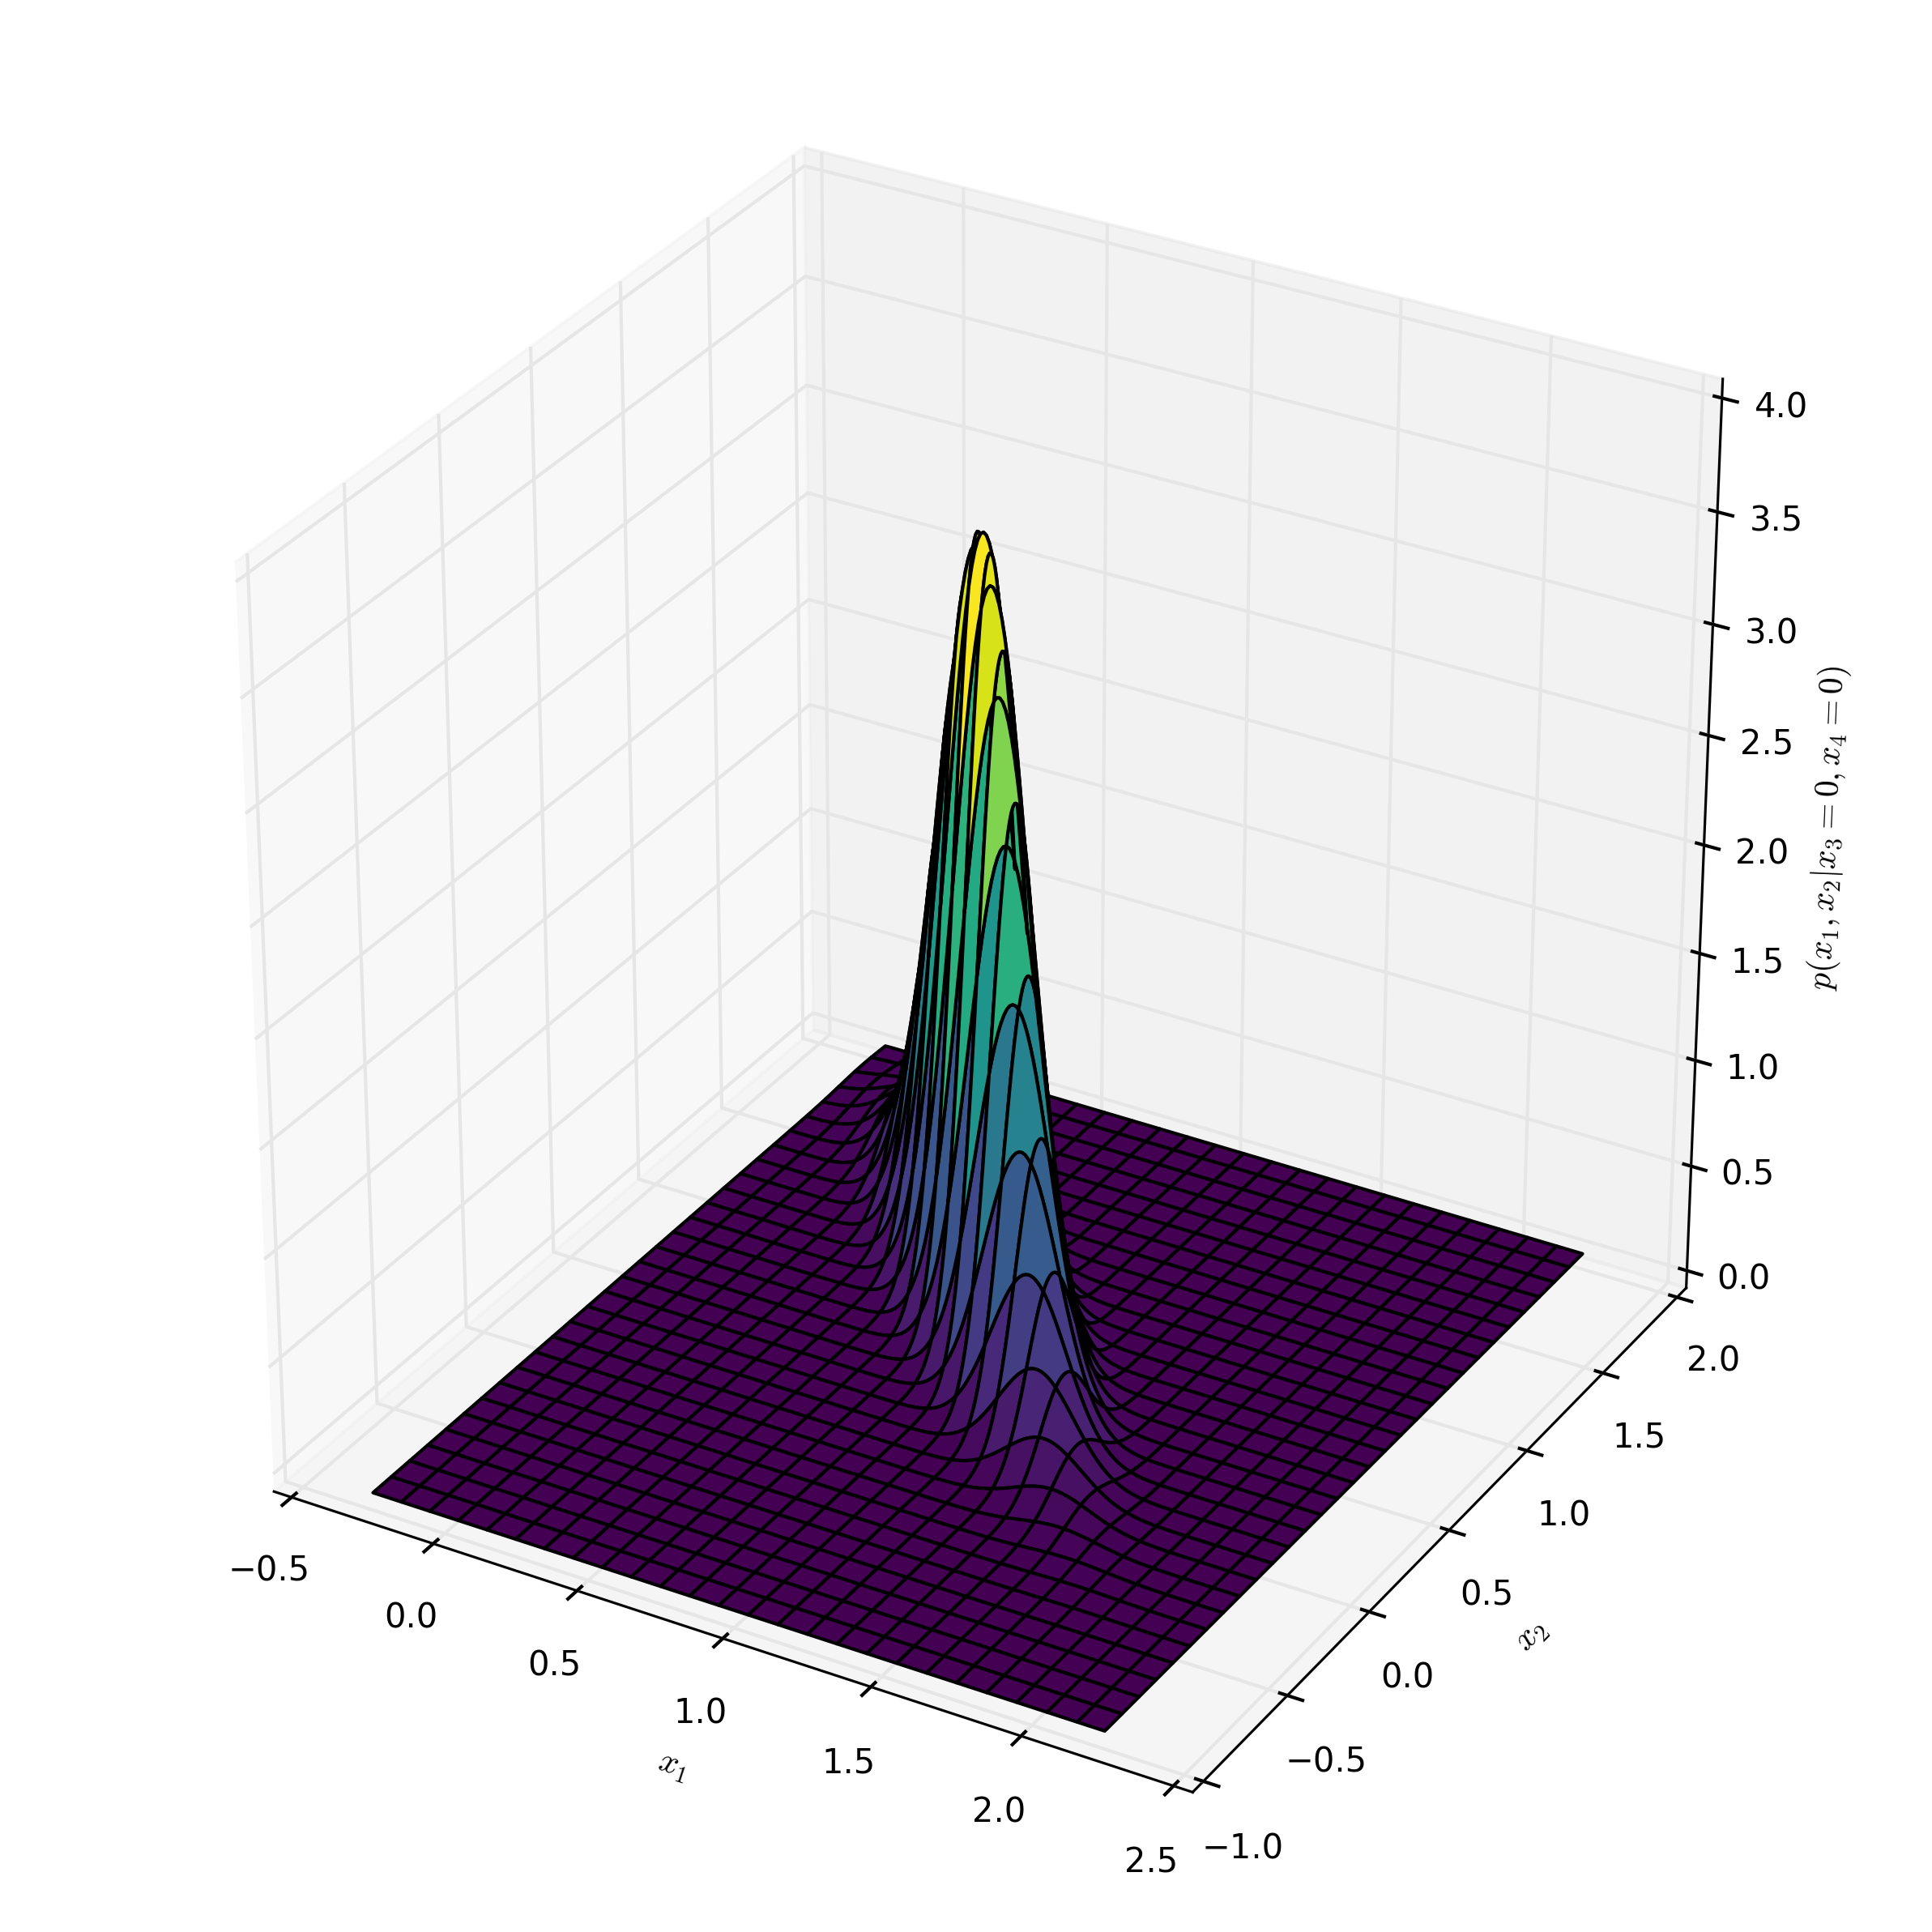
\includegraphics[width=\textwidth]{images/cond_mvg.png}
\caption{Probability density plot of the multivariate Gaussian}
\label{fig:cond_mvg}
\end{figure}
\end{enumerate}
\pagebreak
\subsection*{Part 2 -- Generating the data}
\begin{enumerate}
\item 
\begin{python}
N = 1000
data = np.random.multivariate_normal([0.28, 1.18], 
				     [[2.0, 0.8], 
				      [0.8, 4.0]], 
				     N)
np.savetxt('data.txt', data)
\end{python}
\item The maximum likelihood estimate of the mean is simply the mean of the observed data:
$$
\bm{\mu}_\text{ML} = \frac{1}{N}\sum_{n=1}^N\bm{x}_n = \begin{pmatrix}0.25 \\ 1.21 \end{pmatrix}
$$
Computing the maximum likelihood estimate of the covariance is slightly more involved:
$$
\bm{\Sigma}_\text{ML} = \frac{1}{N}\sum_{n=1}^N(\bm{x}_n - \bm{\mu}_\text{ML})(\bm{x}_n - \bm{\mu}_\text{ML})^T = 
\begin{pmatrix}
2.023 & 0.828 \\
0.828 & 3.626
\end{pmatrix}
$$
To compute the unbiased maximum likelihood covariance estimate, we normalize by $N - 1$ instead of $N$:
$$
\bm{\Sigma}_\text{ML} = \frac{1}{N - 1}\sum_{n=1}^N(\bm{x}_n - \bm{\mu}_\text{ML})(\bm{x}_n - \bm{\mu}_\text{ML})^T = 
\begin{pmatrix}
2.025 & 0.829 \\
0.829 & 3.629
\end{pmatrix}
$$
These results were obtained with the following code:
\begin{python}
mu_ml = data.mean(axis=0)
x = data - mu_ml
cov_ml = np.dot(x.T, x) / N
cov_ml_unbiased = np.dot(x.T, x) / (N - 1)
\end{python}
Note that the left factor is transposed instead of the right factor in the covariance estimates. This is because our points are row vectors instead of column vectors (i.e., \texttt{data} has shape $N \times 2$).

\par We can compare our estimates to the true statistics:
$$
\bm{\mu}_t = \begin{pmatrix} 0.28 \\ 1.18\end{pmatrix} \hspace{2em} \bm{\Sigma}_t = \begin{pmatrix} 2.0 & 0.8 \\ 0.8 & 4.0 \end{pmatrix}
$$
Our estimates are pretty close to their true values. The unbiased estimate of the covariance is not much closer than the biased estimate. Because N is relatively high, the slight change in normalization does not have much effect.
\end{enumerate}
\pagebreak
\subsection*{Part 3 -- Sequential learning algorithms}
\begin{enumerate}
\item Using equation 2.126 from Bishop
$$
\bm{\mu}_\text{ML}^{(N)} = \bm{\mu}_\text{ML}^{(N-1)} + \frac{1}{N}(\bm{x}_N - \bm{\mu}_\text{ML}^{(N-1)})
$$
we can come up with a Python procedure for sequential learning:
\begin{python}
mu_ml = 0
for i in range(N):
    mu_ml += (data[i]-mu_ml) / (i+1)
\end{python}
The starting value $\bm{\mu}_\text{ML}^{(0)}$ does not matter, but is arbitrarily set to 0. We divide by $i + 1$ instead of just $i$, because Python uses 0-indexing.
\item 
\end{enumerate}
\end{document}